\documentclass[12pt]{article}
\usepackage[utf8]{inputenc}
\usepackage{subcaption}  
\usepackage{graphicx}
\usepackage{float}
\usepackage{geometry}
\usepackage{amsmath}
\usepackage{amssymb}
\usepackage{xcolor}
\usepackage{lipsum} % For placeholder text

\geometry{a4paper, margin=1in}
\pagestyle{empty} % No page numbers

\begin{document}

% ===================================================================
% PAGE 1: CLASSIFICATION NOTICE
% ===================================================================
\begin{center}
    \vspace*{1cm}
    {\Huge \textbf{\textcolor{red}{TOP SECRET // FOR INTERNAL USE ONLY}}}
    
    \vspace{2cm}
    \fbox{\parbox{0.8\textwidth}{
        \centering
        \Large \textbf{CLASSIFICATION NOTICE} \\
        \vspace{0.5cm}
        \normalsize
        This document contains proprietary and confidential information pertaining to advanced research and development. The information is the exclusive property of the project lead and associated institution.
        
        \vspace{0.5cm}
        Unauthorized access, reproduction, distribution, or disclosure of this material, in whole or in part, is strictly prohibited. Violators will be subject to the fullest extent of applicable institutional and civil policies.
        
        \vspace{0.5cm}
    }}
    
 

    \vspace{3cm}
    \begin{tabular}{ll}
        \textbf{STUDENT NAME:} & S. HARI PREETHAM \\
        \textbf{SUPERVISING AUTHORITY:} & DR. A. CHENNAKESAVA REDDY \\
        \textbf{INSTITUTION:} & JNTUH UCESTH \\
    \end{tabular}
    
    \vspace{2cm}
    {\large \textit{Handle with extreme care. Information contained herein is critical to ongoing research objectives.}}

    \vfill
    {\textbf{\textcolor{red}{CONFIDENTIAL}}}
\end{center}

\newpage

% ===================================================================
% PAGE 2: TITLE PAGE
% ===================================================================
\begin{titlepage}
    \centering
    {\Large A Project Report on} \\
    \vspace{1.5cm}
    {\Huge \textbf{
Real-Time Precision Actuation in Laser Steering Systems \\[0.1cm]
via Visual-Inertial Fusion and Active\\[0.3cm] Vibration Compensation
}}

    \vspace{2cm}
    
    {\large Submitted by:} \\
    \vspace{0.5cm}
    {\Large \textbf{S HARI PREETHAM}} \\
    {\large 21011P0329} \\
    \vspace{1.5cm}
    
    {\large Under the Esteemed Guidance of} \\
    \vspace{0.5cm}
    {\Large \textbf{DR. A. CHENNAKESAVA REDDY}} \\
    {\large Senior Professor, Department of Mechanical Engineering} \\
    \vfill
    
    % \includegraphics[width=0.3\textwidth]{logo.png} \\
    % \vspace{1cm}
    
    {\Large \textbf{JAWAHARLAL NEHRU TECHNOLOGICAL \\[0.1cm] UNIVERSITY HYDERABAD}} \\
    \vspace{0.2cm}
    {\large UNIVERSITY COLLEGE OF ENGINEERING SCIENCE AND TECHNOLOGY, HYDERABAD} \\ [0.1cm]
    \vspace{1.5cm}
    
    {\large August 2025}
\end{titlepage}

% ===================================================================
% TABLE OF CONTENTS
% ===================================================================
\pagestyle{plain}
\pagenumbering{roman} % Use roman numerals (i, ii, iii) for front matter
\tableofcontents
\newpage
\pagenumbering{arabic} % Switch back to arabic numerals (1, 2, 3) for the main document

% ===================================================================
% PAGE 3: ABSTRACT, PROBLEM STATEMENT, NOVELTY
% ===================================================================
\pagestyle{plain} % Enables page numbering (e.g., 1, 2, 3...)
\setcounter{page}{1} % Resets the page counter to start at 1

\section*{Abstract}

Conventional laser-based weeding systems, while a promising chemical-free alternative in precision agriculture, rely on high-mass platforms with passive mechanical isolation. This brute-force approach to stabilization necessitates the use of high-power pulsed lasers, which significantly increases the system's cost, complexity, safety concerns, and energy requirements.

This project proposes a low-cost, lightweight, control-centric paradigm: an active vibration compensation framework engineered from salvaged mechatronic components. The system integrates both inertial (IMU) and vision-based feedback to dynamically track and eliminate line-of-sight (LOS) jitter in real-time. This active stabilization enables the effective use of safe, low-power, continuous-wave (CW) lasers. Custom galvanometers, constructed from repurposed Hard-Disk Drive (HDD) and optical drive actuators, are governed by high-bandwidth control systems (PID, LQR, MPC). These controllers are based on state-space models derived from experimental system identification and Kalman filtering.

To complement the core stabilization, a computer vision pipeline is implemented for real-time plant versus weed classification and tracking, utilizing pre-trained deep learning models such as YOLOv8 for detection and DeepSORT/ByteTrack for object tracking. This enables robust visual servoing, locking the laser onto dynamic weed targets even under significant platform motion. While the primary application domain is agricultural automation, the core innovation—high-fidelity stabilization via hybrid sensor fusion and AI-guided control—is fundamental to defense, aerospace, and medical robotics.

\vspace{1cm}

\section*{Problem Statement and Motivation}

The deployment of precision laser systems on mobile platforms is severely hampered by several key challenges that current solutions fail to adequately address:
\begin{itemize}
    \item \textbf{Prohibitive Cost and Bulk:} Existing laser steering platforms depend on high-end, laboratory-grade galvanometers or heavy, complex gimbal mechanisms. These systems are expensive, bulky, and unsuitable for lightweight, cost-sensitive mobile applications like agricultural robots.
    \item \textbf{Unaddressed Mechanical Disturbance:} The majority of existing systems are designed for stationary or mechanically isolated platforms. The critical problem of maintaining real-time pointing accuracy under dynamic disturbances (e.g., vehicle vibration, terrain-induced movement) remains largely under-explored.
    \item \textbf{Lack of Sensor Fusion for Beam Control:} While sensor fusion is ubiquitous in navigation and robotics, its specific application to real-time beam steering and actuation control is a nascent field. There is a significant gap in integrating visual and inertial data to directly compensate for beam deviation.
    \item \textbf{Absence of Real-World Performance Metrics:} The literature lacks systematic experimental evaluation of actuation accuracy under vibration. Key performance metrics such as jitter suppression, settling time, and overshoot on disturbed platforms are not well-studied, making it difficult to compare system efficacy.
\end{itemize}

\vspace{1cm}

\section*{Novelty and Contribution}

This project makes several novel contributions to the field of mechatronics and control systems:
\begin{itemize}
    \item \textbf{Resource-Constrained Mechatronics:} It demonstrates that low-cost, salvaged hardware from e-waste can achieve high-precision control performance when coupled with modern software techniques, offering a viable alternative to expensive off-the-shelf components.
    \item \textbf{Hybrid AI + Control Stack:} It pioneers the integration of deep-learning-based computer vision with classical and modern control theory (PID, LQR, MPC) for active visual servoing in a precision actuation context.
    \item \textbf{Visual-Inertial Fusion for Disturbance Rejection:} It applies cutting-edge mapping and localization concepts (Visual-Inertial SLAM) not for navigation, but as a core component of a disturbance rejection framework for a dynamic targeting system.
    \item \textbf{Broad Impact Framework:} The core disturbance rejection and active stabilization framework is domain-agnostic and directly applicable to other high-stakes fields, including aerospace (satellite laser communication), defense (target tracking, counter-UAV systems), and medical optics.
\end{itemize}

\newpage


% ===================================================================
% CHAPTER 2: THEORETICAL FRAMEWORK
% ===================================================================
\section{Theoretical Framework}

The ability to precisely and rapidly steer a laser beam requires a robust mathematical model of the system's mechanics and optics.
 This section develops this framework, beginning with the fundamental laws of reflection and culminating in the kinematic models that translate desired target coordinates into physical actuator commands.

\subsection{Principle of Reflection and the 2\(\theta\) Rule}

The kinematic model is built upon the law of reflection. A critical and direct consequence for dynamic systems is the 2\(\theta\) Rule: a mechanical rotation of a mirror by an angle \(\theta\) deflects the reflected optical path by \(2\theta\).

This angular amplification is a direct result of the geometry.
 When the mirror plane rotates by \(\theta\), the mirror's normal vector must also rotate by the same angle
  \(\theta\). This rotation changes the angle of incidence by \(\theta\). To satisfy the law of reflection
  with respect to this new normal, the angle of reflection must also change by \(\theta\).
   The total deflection is the sum of these two changes, resulting in a robust and predictable deflection 
   of precisely \(2\theta\). This effect provides a crucial mechanical advantage, allowing small, 
   high-speed rotations to produce a large angular sweep of the laser beam.


\subsubsection{A First Approximation: Planar Projection}
As a first-order model for a single-axis scanner, we can directly apply the 2\(\theta\) rule using basic trigonometry. Consider a single mirror pivoting at the origin and deflecting a laser beam onto a flat screen positioned at a perpendicular distance \(d\).

The optical deflection angle is \(2\theta\). In the right-angled triangle formed by the pivot point, the center of the screen, and the laser spot, the displacement of the spot (\(x\)) is the side opposite to this angle. Therefore, the relationship is given by:
\begin{equation}
    \tan(2\theta) = \frac{\text{opposite}}{\text{adjacent}} = \frac{x}{d}
\end{equation}
Solving for the displacement \(x\) gives our first approximation:
\begin{equation}
    x = d \tan(2\theta)
\end{equation}
While simple and useful for basic estimations, this model is insufficient for a high-fidelity 2D system because it fails to account for the sequential reflections and the physical distance between the two mirrors. For a rigorous model, we must therefore use the vector form of reflection.


\begin{figure}[H]
    \centering
    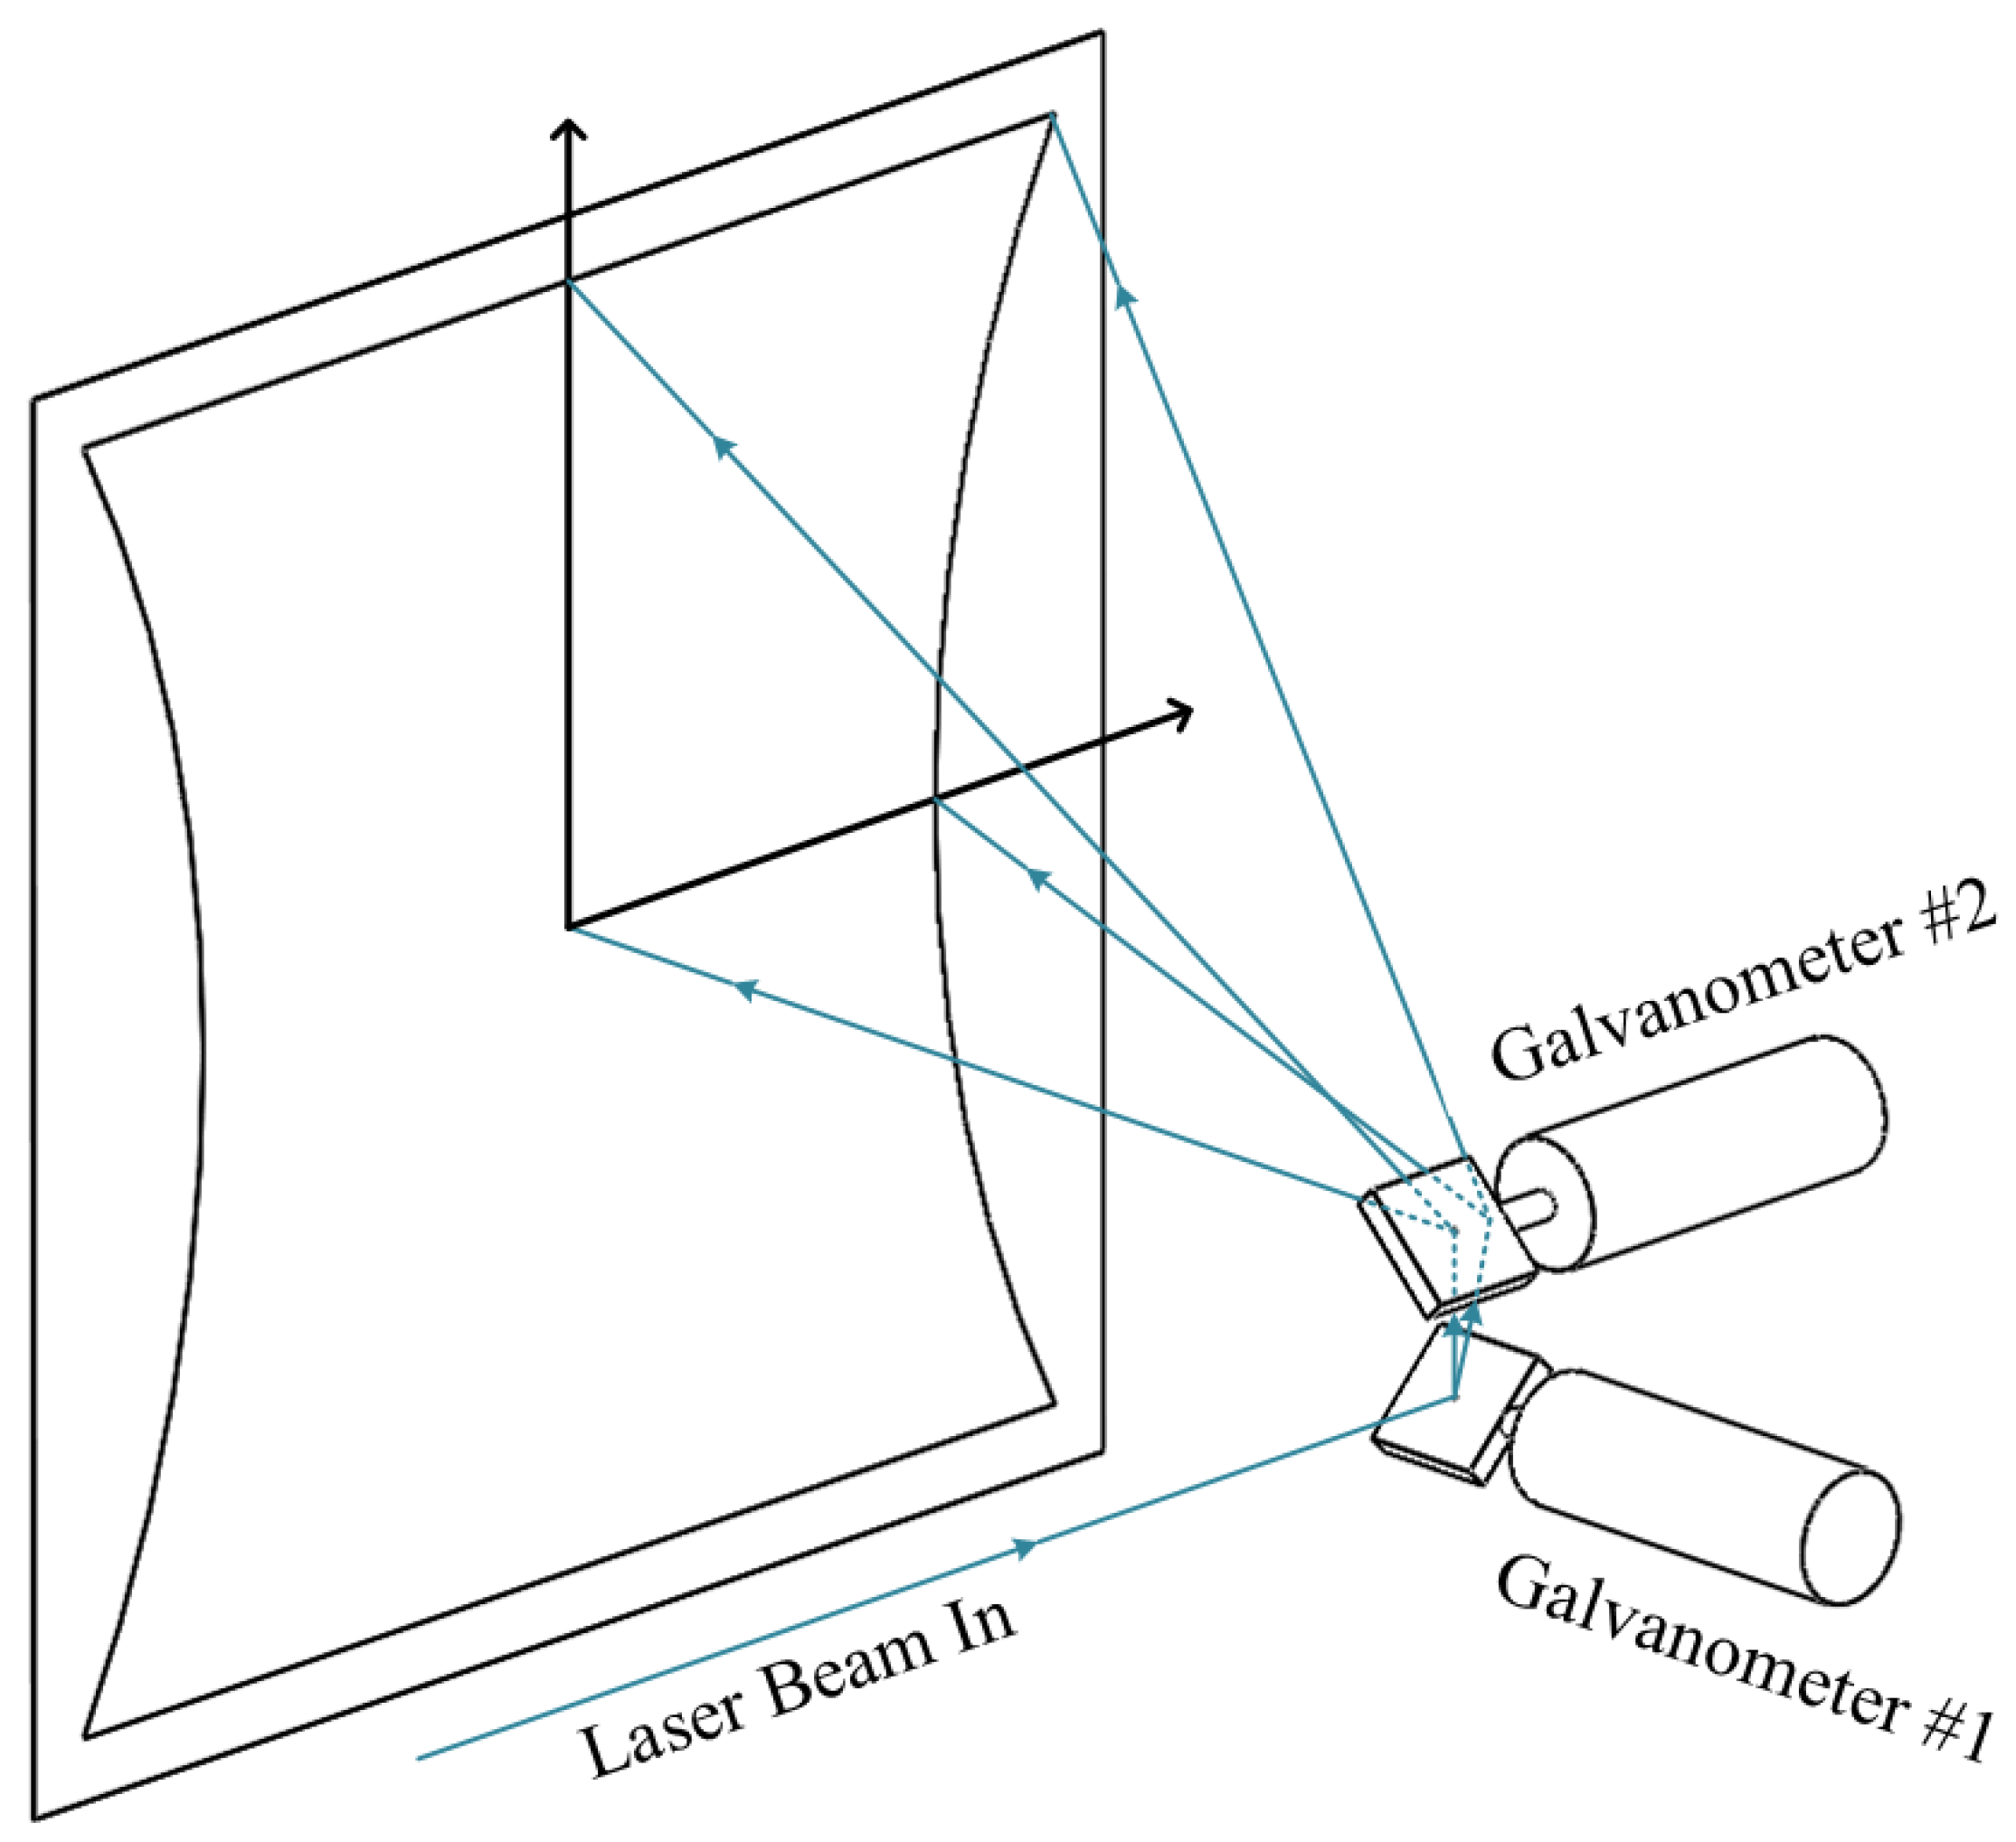
\includegraphics[width=0.7\textwidth]{./images/optics_of_galvo_scanner.png} % replace with your file name
    \caption{Geometric illustration of the principle of reflection and the $2\theta$ rule.}
    \label{fig:reflection_2theta}
\end{figure}

Therefore, by using a dual-axis galvanometer setup, the laser beam can be directed to any point within a defined area on the X–Y plane. The size of this area is determined by the mirror dimensions, the angular range of rotation, and the distance between the mirror system and the projection surface.     
\subsubsection{Vector Form of Reflection}
Let \(\vec{V}\) be the unit vector representing the direction of the incoming laser beam, and let \(\vec{N}\) be the unit normal vector of the mirror surface. The resulting reflected vector, \(\vec{R}\), is given by:
\begin{equation}
    \vec{R} = \vec{V} - 2(\vec{V} \cdot \vec{N})\vec{N}
    \label{eq:vector_reflection}
\end{equation}
This equation forms the basis of our kinematic model. 

\subsection{Forward Kinematics: From Mirror Angles to Screen Coordinates}

Forward kinematics provides a mathematical model to calculate the final laser spot position on the screen, \((X_f, Y_f)\), from a given set of mechanical mirror angles, \((\theta_x, \theta_y)\). To construct this model, we first define a standard 3D Cartesian coordinate system:

\begin{itemize}
\item The origin, \([0,0,0]\), is defined as the pivot center of the first mirror (the X-mirror).
\item The \textbf{Z-axis} represents the path of the incoming laser beam.
\item The \textbf{X-mirror} is responsible for horizontal deflection. It pivots around the \textbf{Y-axis} by a mechanical angle \(\theta_y\).
\item The \textbf{Y-mirror} is responsible for vertical deflection. It is positioned at a distance \(e\) along the X-axis from the first mirror. It pivots around an axis parallel to the \textbf{X-axis} by a mechanical angle \(\theta_x\).
\end{itemize}

The initial state is an incoming laser beam traveling along the Z-axis, represented by the vector \(\vec{V}_{in} = [0, 0, 1]^T\). The undeflected normals of the mirrors, \(\vec{N}_{x0}\) and \(\vec{N}_{y0}\), are typically oriented at 45 degrees to the Z-axis to correctly fold the optical path.

A rotation of a mirror changes its normal vector. The new normal is found by applying a 3D rotation matrix to the initial normal vector.
\begin{itemize}
\item \textbf{Rotation around X-axis} (for Y-mirror, angle \(\theta_x\)):
\begin{equation}
\mathbf{R}_x(\theta_x) = \begin{bmatrix} 1 & 0 & 0 \\ 0 & \cos\theta_x & -\sin\theta_x \\ 0 & \sin\theta_x & \cos\theta_x \end{bmatrix}
\end{equation}
\item \textbf{Rotation around Y-axis} (for X-mirror, angle \(\theta_y\)):
\begin{equation}
\mathbf{R}_y(\theta_y) = \begin{bmatrix} \cos\theta_y & 0 & \sin\theta_y \\ 0 & 1 & 0 \\ -\sin\theta_y & 0 & \cos\theta_y \end{bmatrix}
\end{equation}
\end{itemize}

\subsubsection{Full Path Algorithm}
The final direction of the laser beam is calculated through a sequence of two reflections:
\begin{enumerate}
\item \textbf{First Reflection (X-mirror):} The X-mirror's normal vector is updated based on its rotation: \(\vec{N}_{x} = \mathbf{R}_y(\theta_y)\vec{N}_{x0}\). The incoming beam reflects off this surface, resulting in a new direction vector: \(\vec{R}_1 = \vec{V}_{in} - 2(\vec{V}_{in} \cdot \vec{N}_{x})\vec{N}_{x}\). The components of \(\vec{R}_1\) are now trigonometric functions of the angle \(\theta_y\).
\item \textbf{Second Reflection (Y-mirror):} The Y-mirror's normal vector is similarly updated: \(\vec{N}_{y} = \mathbf{R}_x(\theta_x)\vec{N}_{y0}\). The beam from the first mirror, \(\vec{R}_1\), is the incoming vector for this reflection. The final direction vector is therefore: \(\vec{R}_{final} = \vec{R}_1 - 2(\vec{R}_1 \cdot \vec{N}_{y})\vec{N}_{y}\).
\end{enumerate}
It is critical to note that during this second reflection, the dot product term \((\vec{R}_1 \cdot \vec{N}_{y})\) mathematically entangles the two rotation angles. Because \(\vec{R}_1\) is a function of \(\theta_y\) and \(\vec{N}_{y}\) is a function of \(\theta_x\), the resulting vector \(\vec{R}_{final}\) contains complex, non-linear cross-coupled terms, making it impossible to separate the influence of each angle cleanly.

\subsubsection{Ray-Plane Intersection and Pincushion Distortion}
With the final direction vector \(\vec{R}_{final} = [R_x, R_y, R_z]^T\), we can determine its intersection with a screen plane. The final ray originates from the pivot point of the Y-mirror, which is located at \(\vec{P}_y = [e, 0, 0]^T\). The parametric equation for this ray is \(\vec{P}(t) = \vec{P}_y + t \cdot \vec{R}_{final}\).

The screen is a plane defined by the equation \(z=d\), where \(d\) is the perpendicular distance from the Y-mirror's pivot axis to the screen. To find the intersection point, we solve the z-component of the parametric equation for the parameter \(t\):
\begin{equation}
0 + t \cdot R_z = d \implies t = \frac{d}{R_z}
\end{equation}
Substituting \(t\) back into the x and y components gives the final coordinates \((X_f, Y_f)\):
\begin{equation}
X_f = e + t \cdot R_x = e + d \frac{R_x}{R_z}
\end{equation}
\begin{equation}
Y_f = 0 + t \cdot R_y = d \frac{R_y}{R_z}
\end{equation}
This model fully describes the geometry of the system. It also reveals the source of pincushion distortion. The final X-coordinate depends not just on its own angle but also on the path length to the screen. This path length is modulated by the tilt of the Y-mirror, causing the scan field to become wider at the top and bottom edges, which creates the characteristic pincushion shape.

\subsubsection{Matrix Representation of the Kinematic Chain}

To more clearly illustrate the coupling between the mirror rotations, we can represent the reflection operation itself as a matrix transformation. For a given mirror normal \(\vec{N}\), the reflection matrix \(\mathbf{M}_{ref}(\vec{N})\) that transforms an incoming vector \(\vec{V}\) to a reflected vector \(\vec{R}\) is given by:

\begin{equation}
\mathbf{M}_{ref}(\vec{N}) = \mathbf{I} - 2(\vec{N} \otimes \vec{N}) = \begin{bmatrix} 1 - 2N_x^2 & -2N_xN_y & -2N_xN_z \\ -2N_xN_y & 1 - 2N_y^2 & -2N_yN_z \\ -2N_xN_z & -2N_yN_z & 1 - 2N_z^2 \end{bmatrix}
\end{equation}
where \(\mathbf{I}\) is the identity matrix and \(\otimes\) denotes the outer product.

Using this representation, the entire forward kinematic chain can be expressed as a single composite transformation matrix, \(\mathbf{M}_{total}\), acting on the initial beam vector:

\begin{enumerate}
\item The reflection matrix for the X-mirror, \(\mathbf{M}_{ref,X}\), is a function of its normal, \(\vec{N}_x\), which in turn depends on the angle \(\theta_y\).
\item The reflection matrix for the Y-mirror, \(\mathbf{M}_{ref,Y}\), is a function of its normal, \(\vec{N}_y\), which depends on the angle \(\theta_x\).
\item The final direction vector is therefore given by the product of these matrices:
\begin{equation}
\vec{R}_{final} = \mathbf{M}_{ref,Y}(\theta_x) \cdot \mathbf{M}_{ref,X}(\theta_y) \cdot \vec{V}_{in}
\end{equation}
\end{enumerate}

This formulation makes the "entanglement" explicit. The total transformation matrix is the product of two matrices, each dependent on one of the control angles. Because matrix multiplication is not commutative \((\mathbf{A}\mathbf{B} \neq \mathbf{B}\mathbf{A})\), the final result is a complex function where the influences of \(\theta_x\) and \(\theta_y\) are thoroughly mixed. This elegantly demonstrates why a simple, separable analytical solution for the inverse kinematics is not possible.

\subsection{Inverse Kinematics: The Challenge of Target-to-Angle Mapping}

For any practical control application, we must solve the inverse problem: given a desired target on the screen \((X_{target}, Y_{target})\), what are the required mirror angles \((\theta_x, \theta_y)\)? This is the inverse kinematics (IK) problem.

The forward kinematic model, while accurate for simulation, is insufficient for real-time control, especially on a mobile platform, because:
\begin{itemize}
\item The reference frame is no longer static; the entire scanner assembly, including the mirror pivots and the screen plane, is moving and vibrating relative to the world.
\item The system must solve for angles in real-time to track a target, compensating for both the target's position and the platform's own motion.
\item As demonstrated, the forward mapping \((X_f, Y_f) = f(\theta_x, \theta_y)\) is a complex, non-linear, and coupled function. A direct analytical inversion to find \((\theta_x, \theta_y) = f^{-1}(X_f, Y_f)\) is mathematically intractable for a real-time system.
\end{itemize}

\subsubsection{Analytical vs. Numerical IK}
An \textbf{analytical} solution would provide a direct, closed-form equation, e.g., \(\theta_x = f(X,Y)\). While derivable for highly simplified cases (e.g., assuming perfectly orthogonal, co-located mirrors), such solutions are brittle and fail to account for real-world mechanical realities, rendering them useless for a high-precision system.

A \textbf{numerical} solution iteratively finds the angles. This approach is more robust and can adapt to complex, non-ideal systems, which is essential for our application. We use the Jacobian-based iterative method.

\subsection{Numerical Solution: The Jacobian Iterative Method}

The Jacobian matrix, \(\mathbf{J}\), serves as a "sensitivity map." It relates infinitesimal changes in the input (mirror angles) to the resulting infinitesimal changes in the output (screen position). It is the matrix of all first-order partial derivatives of the forward kinematics function:
\begin{equation}
    \mathbf{J}(\boldsymbol{\theta}) = \begin{bmatrix} \frac{\partial X_f}{\partial \theta_x} & \frac{\partial X_f}{\partial \theta_y} \\ \frac{\partial Y_f}{\partial \theta_x} & \frac{\partial Y_f}{\partial \theta_y} \end{bmatrix}
\end{equation}
where \(\boldsymbol{\theta} = [\theta_x, \theta_y]^T\).

We use this matrix in an iterative algorithm to converge on the correct angles.

\subsubsection{Iterative Inverse Kinematic Algorithm}
\begin{enumerate}
    \item \textbf{Initialization (Step 0):} Identify the target position \(\vec{P}_{target} = [X_{target}, Y_{target}]^T\). Start with the current measured angles of the motors, \(\boldsymbol{\theta}_{current}\).
    \item \textbf{Calculate Current Position (Step 1):} Use the forward kinematics model to calculate the current laser position on the screen, \(\vec{P}_{current}\), based on \(\boldsymbol{\theta}_{current}\).
    \item \textbf{Find the Error (Step 2):} Calculate the error vector between the target and current position: \(\vec{e} = \vec{P}_{target} - \vec{P}_{current}\).
    \item \textbf{Calculate Jacobian (Step 3):} Compute the Jacobian matrix \(\mathbf{J}\) at the current angle configuration \(\boldsymbol{\theta}_{current}\).
    \item \textbf{Determine Angle Correction (Step 4):} The desired change in angles, \(\Delta\boldsymbol{\theta}\), can be found by "inverting" the Jacobian relationship \(\vec{e} \approx \mathbf{J} \Delta\boldsymbol{\theta}\). Instead of using a direct and potentially unstable inverse, we use the Jacobian transpose, which is computationally simpler and more stable:
    \begin{equation}
        \Delta\boldsymbol{\theta} = \alpha \mathbf{J}^T \vec{e}
    \end{equation}
    Here, \(\alpha\) is a small learning rate (a step size) that ensures a stable convergence.
    \item \textbf{Update Guess (Step 5):} Update the motor angles: \(\boldsymbol{\theta}_{new} = \boldsymbol{\theta}_{current} + \Delta\boldsymbol{\theta}\).
    \item \textbf{Repeat:} Set \(\boldsymbol{\theta}_{current} = \boldsymbol{\theta}_{new}\) and repeat from Step 1 until the magnitude of the error vector \(||\vec{e}||\) is below a desired tolerance.
\end{enumerate}
This iterative process allows the system to find the correct angles even for a complex, non-ideal mechanical setup and is the core of the high-level steering control.

\subsubsection{Limitations of the Jacobian Transpose Method}
While computationally efficient, this basic iterative method has a critical flaw for a physical system: it is unconstrained. The algorithm has no inherent knowledge of the galvanometer's mechanical limits. If a target is commanded near or outside the scanner's reachable workspace, this algorithm will calculate and command angles (e.g., \(\theta_x = 15^\circ\)) that are physically impossible for the actuator to achieve. This can lead to actuator saturation, instability, and unpredictable behavior at the edges of the workspace. For a robust, "battle-ready" system, we must be able to handle these physical constraints gracefully.

\subsection{Enhanced Solution: Constrained Optimization}

To address the limitations of the unconstrained approach, we re-frame the IK problem as a formal optimization problem. The goal is no longer just to find *any* solution, but to find the *best possible* solution that satisfies all physical constraints. This is achieved by finding the angle vector \(\vec{\theta}\) that minimizes a scalar Cost Function, \(C(\vec{\theta})\).

\subsubsection{The Cost Function}
The Cost Function mathematically defines the "total error" of the system, balancing pointing accuracy with adherence to physical limits.
\begin{equation}
C(\vec{\theta}) = \frac{1}{2} || \text{FK}(\vec{\theta}) - \vec{P}_{target} ||^2 + \beta H(\vec{\theta}, \vec{\theta}_{max})
\label{eq:cost_function}
\end{equation}

The function consists of two terms:
\begin{itemize}
\item \textbf{Accuracy Term:} \(\frac{1}{2} || \text{FK}(\vec{\theta}) - \vec{P}_{target} ||^2\) is the squared distance error. Minimizing this term drives the laser to the target.
\item \textbf{Constraint Term:} \(H(\vec{\theta}, \vec{\theta}_{max})\) is a \textbf{barrier function} that penalizes angles approaching their limits. A logarithmic barrier is used, which approaches infinity as any angle \(\theta_i\) nears its limit \(\pm\theta_{max}\), creating a "force field" that the optimizer will not violate.
\end{itemize}
The scalar weight \(\beta\) controls the strength of this barrier.

\subsubsection{Solution via Gradient Descent}
The cost function is minimized using the Gradient Descent algorithm, which iteratively updates the angles by taking steps in the direction opposite to the gradient of the cost function.
\begin{equation}
\vec{\theta}_{k+1} = \vec{\theta}_k - \alpha \nabla C(\vec{\theta}_k)
\end{equation}
The gradient \(\nabla C\) is derived from Equation \ref{eq:cost_function} and is composed of the gradient of both the accuracy and the barrier terms. The gradient of the accuracy term is found to be \(\mathbf{J}(\vec{\theta})^T \cdot (\text{FK}(\vec{\theta}) - \vec{P}_{target})\).

\vspace*{0.5cm}

This constrained optimization framework represents the final, robust solution. It leverages the efficiency of the Jacobian while formally incorporating actuator limits. This ensures that the calculated angles are always physically achievable, providing stable and predictable behavior across the entire workspace and preventing the controller from commanding impossible states. This is the core algorithm for the high-level steering controller.

\subsubsection{Algorithm Stability and Convergence}

The stability of the numerical IK solver is a critical consideration. Unlike an analytical solution, an iterative algorithm's performance is not guaranteed and depends on its formulation and tuning.

The proposed algorithm incorporates several features to ensure stable and predictable convergence:

\begin{itemize}
\item \textbf{Use of the Jacobian Transpose:} The choice of the Jacobian Transpose method, \(\Delta\boldsymbol{\theta} = \alpha \mathbf{J}^T \vec{e}\), over a direct matrix inverse, \(\Delta\boldsymbol{\theta} = \mathbf{J}^{-1} \vec{e}\), is a key stabilizing factor. The transpose method is less susceptible to issues with matrix singularities (positions where the inverse is undefined) and generally provides a smoother, more stable path towards the solution, even if it sometimes requires more iterations.

\item \textbf{The Learning Rate (\(\alpha\)):} The scalar step size, \(\alpha\), is a crucial tuning parameter. A small, fixed value for \(\alpha\) will be chosen to prevent the algorithm from taking excessively large steps. This prevents overshooting the target and ensures the iterative process does not become unstable or oscillate.

\item \textbf{Constraint Handling:} The inclusion of the logarithmic barrier function in the constrained optimization framework is another critical stabilizing feature. By preventing the solver from ever commanding angles outside the known physical limits of the actuator, it eliminates a major source of potential instability and ensures all commanded states are physically achievable.`

  

\end{itemize}

\textbf{Verification Method:}
The stability of the implemented algorithm will be verified experimentally. The system will be subjected to a series of step commands to various points within the workspace, including points at the extreme edges. The convergence of the error vector \(||\vec{e}||\) over the iterations will be plotted and analyzed. A stable system will demonstrate a smooth, monotonic decrease in error. Any oscillatory or divergent behavior will be addressed by tuning the learning rate \(\alpha\) and the barrier weight \(\beta\).
\newpage


% ===================================================================
% CHAPTER 3: MECHANICAL DESIGN
% ===================================================================
\section{Mechanical Design and System Architecture}

The efficacy of the laser stabilization and targeting system is fundamentally dependent on the precision, rigidity, and thermal stability of its mechanical architecture. This section details the design of the physical assembly, outlining the system layout, the novel solution for the kinematic mirror mounting, and the rationale behind the material selection and thermal management strategies.

\subsection{System Layout and Kinematic Mounting}

The system is configured as a traditional orthogonal two-axis scanner to produce a Cartesian motion profile. The primary actuators are two Voice Coil Motors (VCMs) salvaged from Hard Disk Drives (HDDs), chosen for their low inertia and high-speed response.

\begin{itemize}
\item The \textbf{X-axis galvanometer assembly} is mounted horizontally onto the main system baseplate. Its pivot axis is oriented vertically (\(Z_{axis}\)).
\item The \textbf{Y-axis galvanometer assembly} is mounted on a rigid, 90-degree vertical support structure. Its pivot axis is oriented horizontally (\(Y_{axis}\)).
\end{itemize}

Unlike commercial galvo scanners, the X-axis mirror subassembly is not a kinematic mount. Instead, it is secured by four M4 bolts with nut–washer sets to a rigid reference platform. Slots are included in the mount to allow linear adjustment of the interface between the X-axis and Y-axis structures. This design provides the flexibility to calibrate the inter-mirror distance for different mirror sizes and optical path requirements, rather than fixing the geometry permanently.

Both X- and Y-axis mounts incorporate embedded hexagonal cavities to seat metal hex nuts within the 3D-printed body. This reinforcement was necessary to withstand the flexural forces imposed by the strong permanent magnets of the HDD actuators. Tolerances in these assemblies are often below 1–2 mm, meaning that even slight deformation of the plastic body would cause misalignment or structural failure. The embedded nut design transfers clamping loads directly into the steel hardware, reducing stress concentration in the printed polymer and improving long-term rigidity.

The Y-axis vertical mount also uses through-holes and embedded nuts to achieve rigid mating with the baseplate, ensuring orthogonality between axes. To compensate for additive manufacturing limitations, the geometry was modified from the original HDD structure. The redesign introduced structural ribs, screw slots, and local thickening in high-stress regions to increase stiffness while keeping the assembly lightweight.
% ================== Part-Level Analysis ==================
\begin{figure}[H]
    \centering
    \begin{subfigure}[b]{0.48\textwidth}
        \centering
        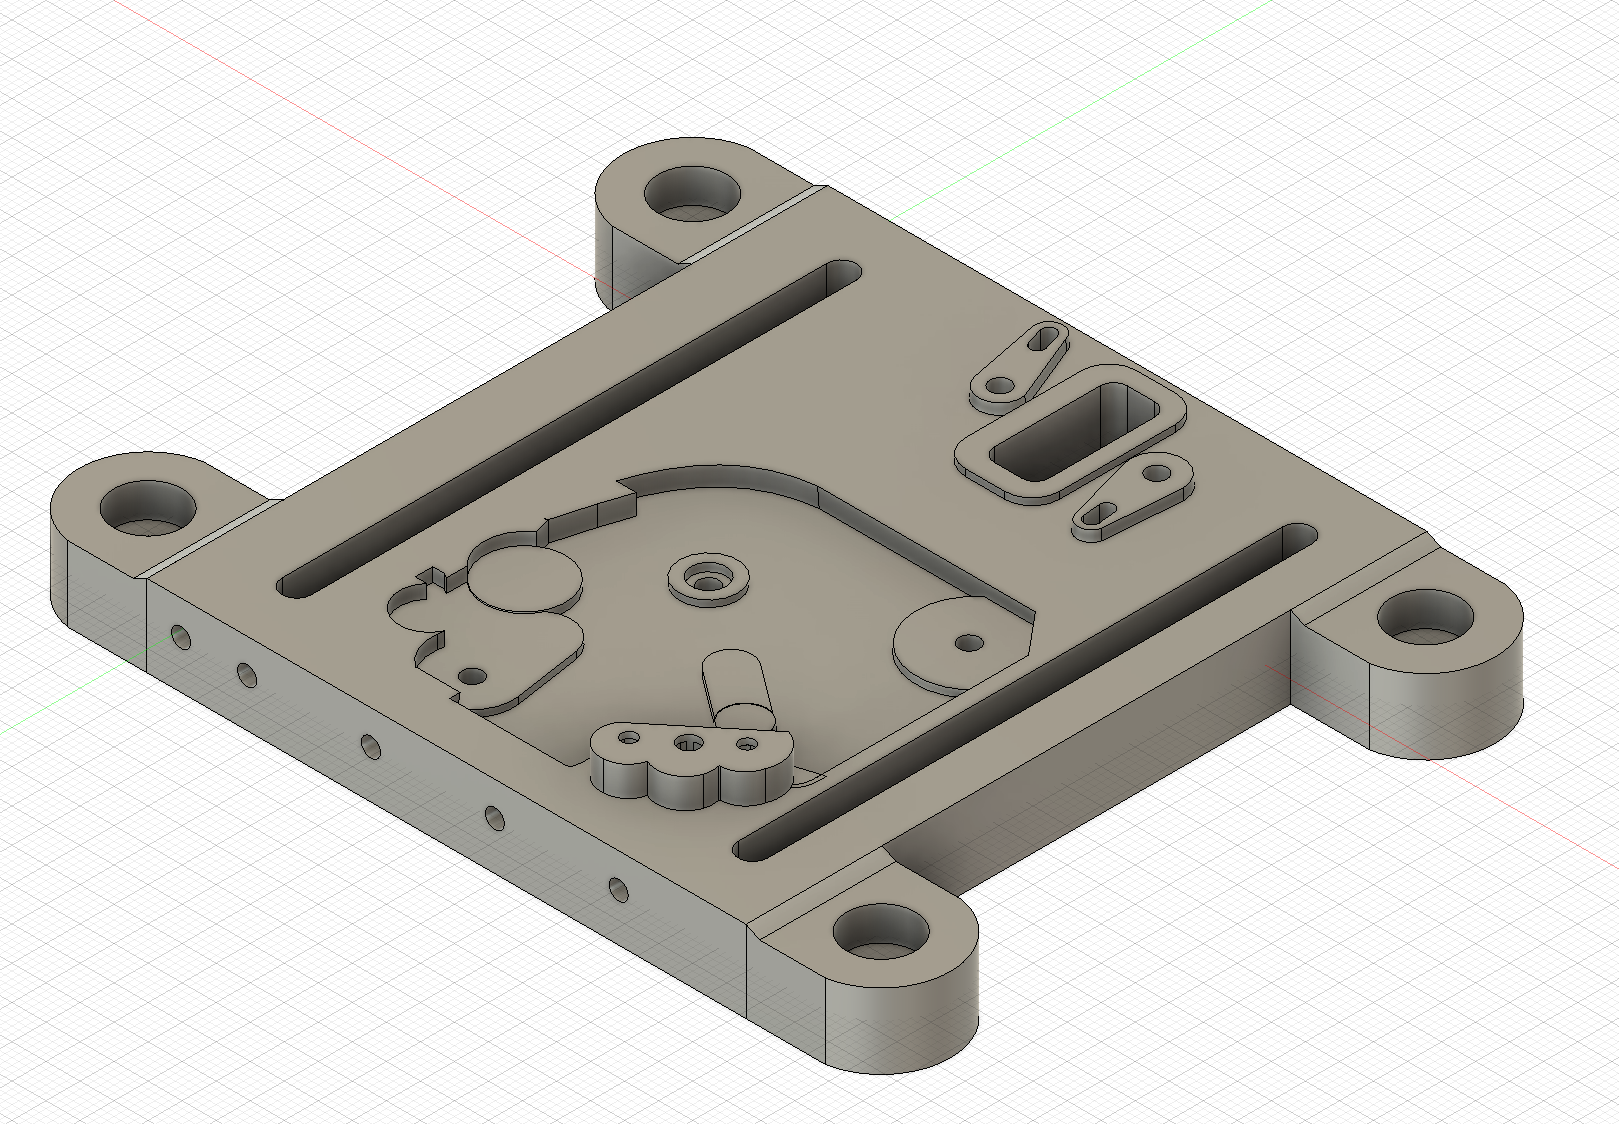
\includegraphics[width=\textwidth]{./images/1.png}
        \caption{X-axis VCM actuator mount}
        \label{fig:x_mount}
    \end{subfigure}
    \hfill
    \begin{subfigure}[b]{0.48\textwidth}
        \centering
        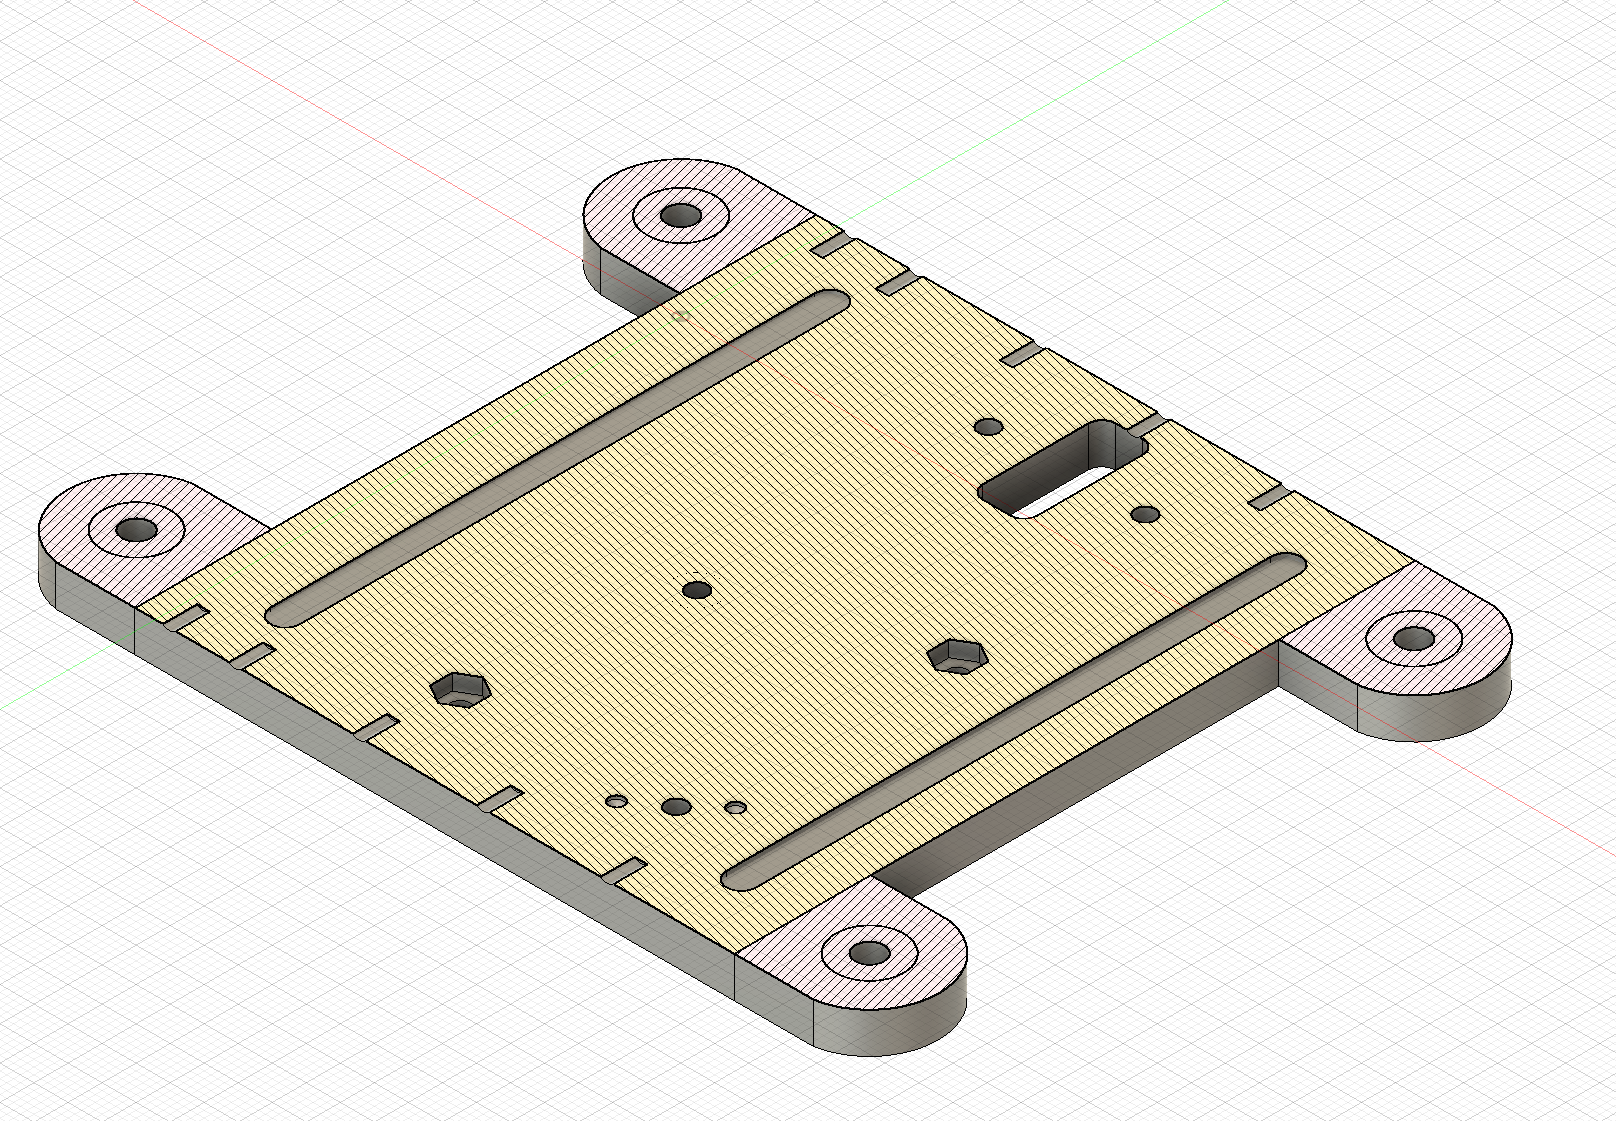
\includegraphics[width=\textwidth]{./images/2.png}
        \caption{Cross-section area analysis of X-axis mount}
        \label{fig:x_cross}
    \end{subfigure}
    \caption{X-axis actuator mount and corresponding cross-section analysis.}
    \label{fig:x_mount_combo}
\end{figure}

\begin{figure}[H]
    \centering
    \begin{subfigure}[b]{0.48\textwidth}
        \centering
        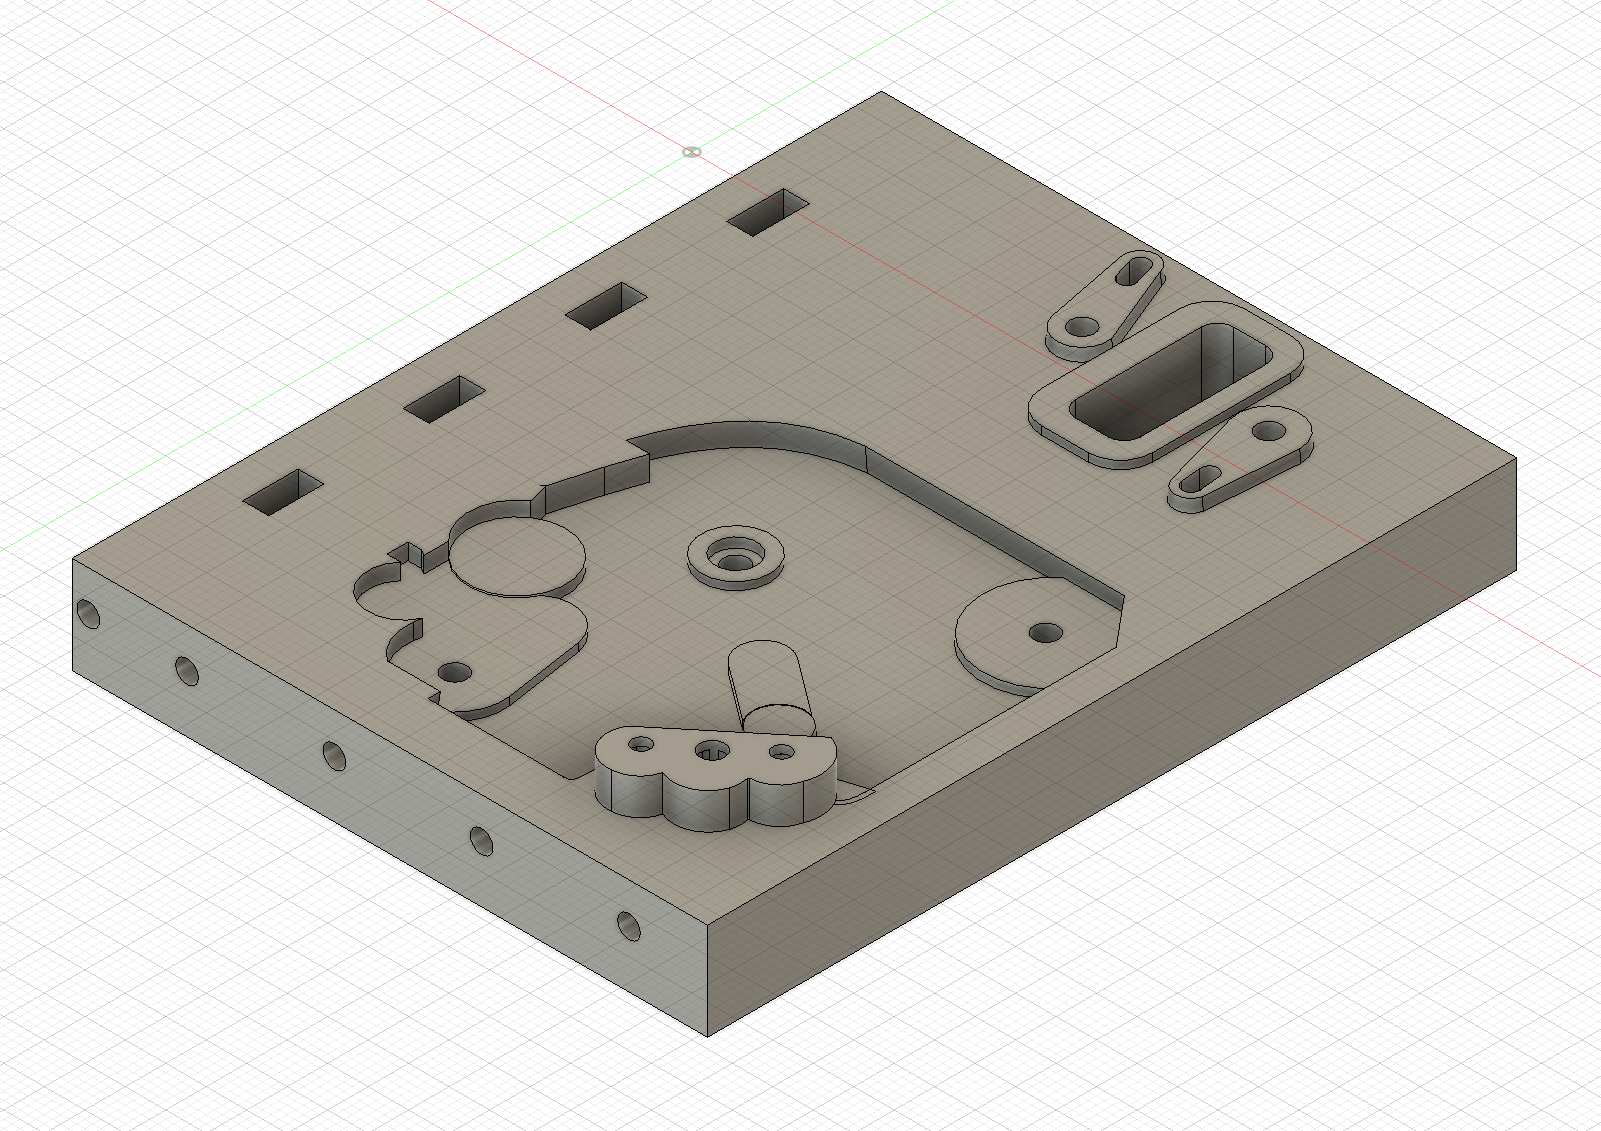
\includegraphics[width=\textwidth]{./images/4.png}
        \caption{Y-axis VCM actuator mount}
        \label{fig:y_mount}
    \end{subfigure}
    \hfill
    \begin{subfigure}[b]{0.48\textwidth}
        \centering
        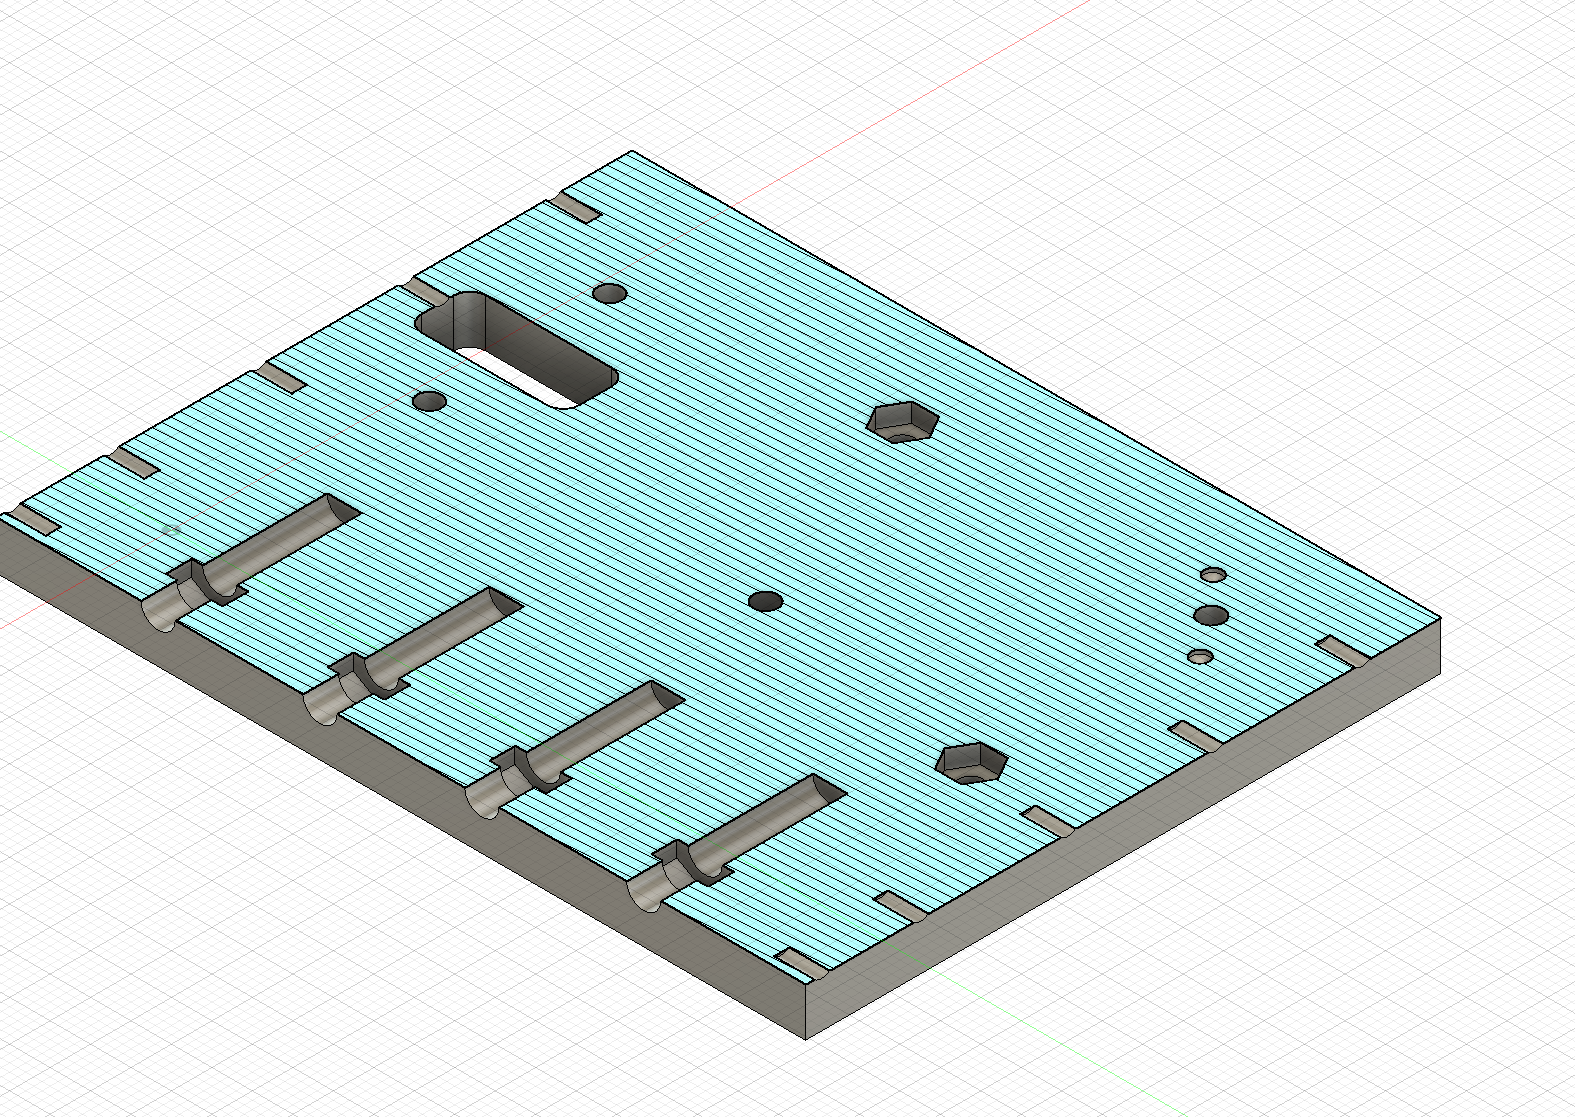
\includegraphics[width=\textwidth]{./images/7.png}
        \caption{Cross-section area analysis of Y-axis mount}
        \label{fig:y_cross}
    \end{subfigure}
    \caption{Y-axis actuator mount and corresponding cross-section analysis.}
    \label{fig:y_mount_combo}
\end{figure}


% ================== Assembly CAD & Structural Analysis ==================
\begin{figure}[H]
    \centering
    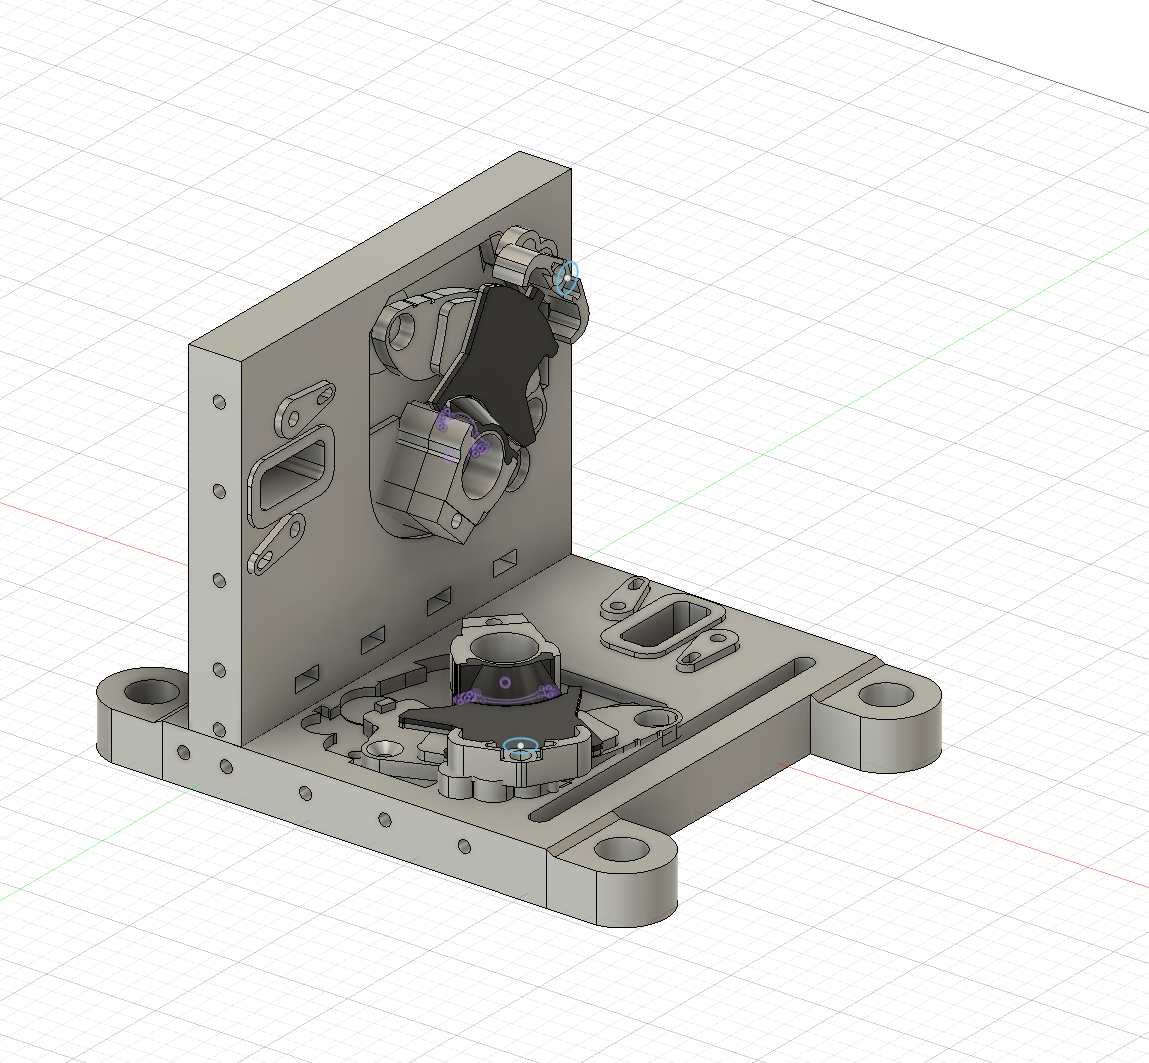
\includegraphics[width=0.95\textwidth]{./images/8.png}
    \caption{CAD model of the complete dual-axis galvanometer assembly, showing orthogonal arrangement of VCM actuators and kinematic mounting points on the main baseplate.}
    \label{fig:assembly_cad}
\end{figure}

\begin{figure}[H]
    \centering
    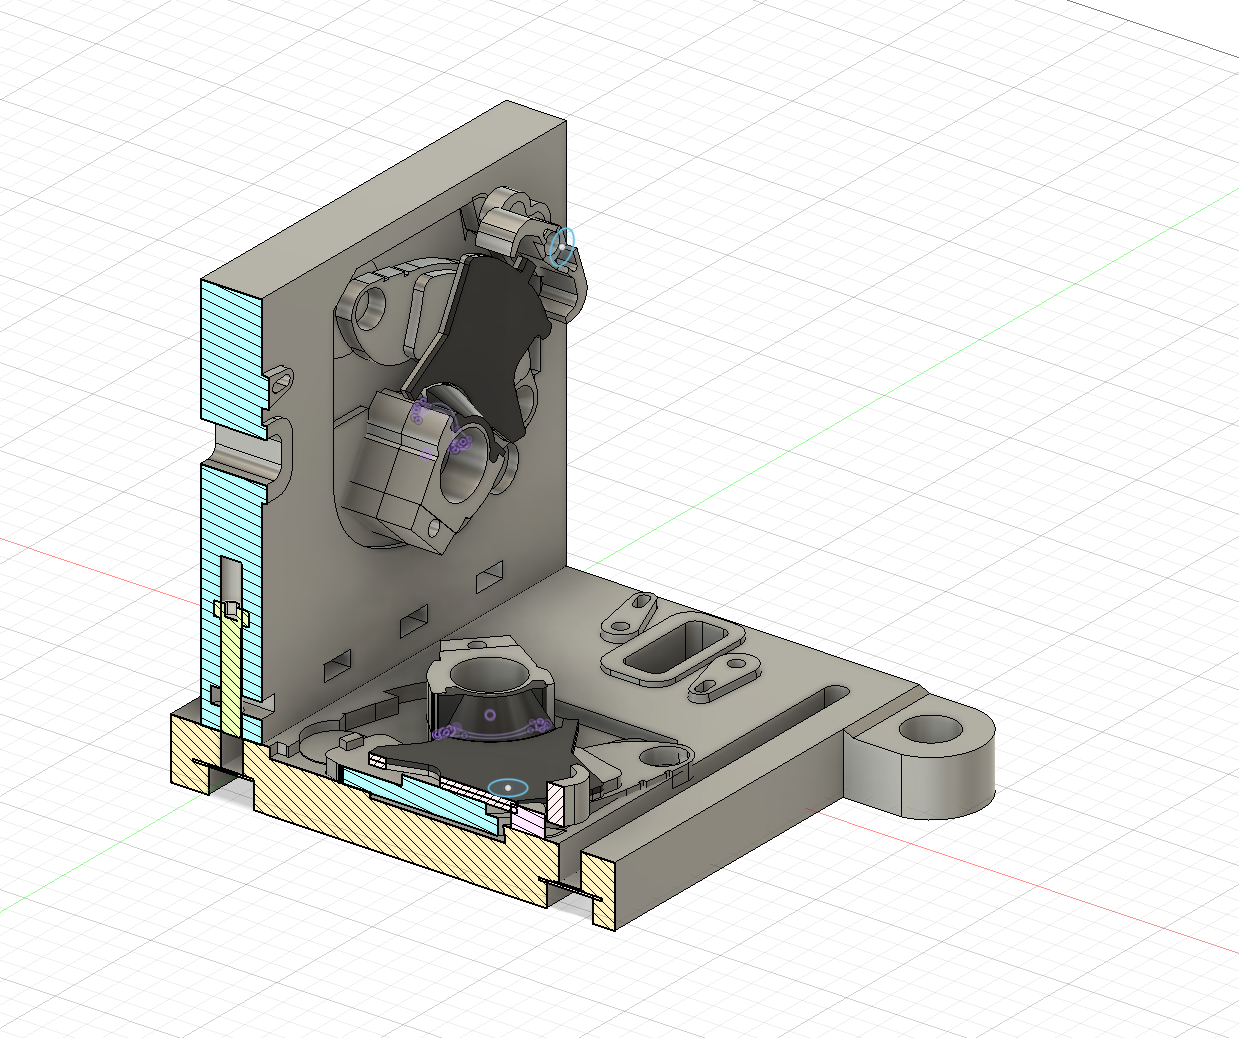
\includegraphics[width=0.95\textwidth]{./images/9.png}
    \caption{Structural cross-section area analysis and mating surfaces of the full assembly. The mounts are fastened using M4 nuts, bolts, and washers.}
    \label{fig:assembly_analysis}
\end{figure}


% ================== Physical Prototype ==================
\begin{figure}[H]
    \centering
    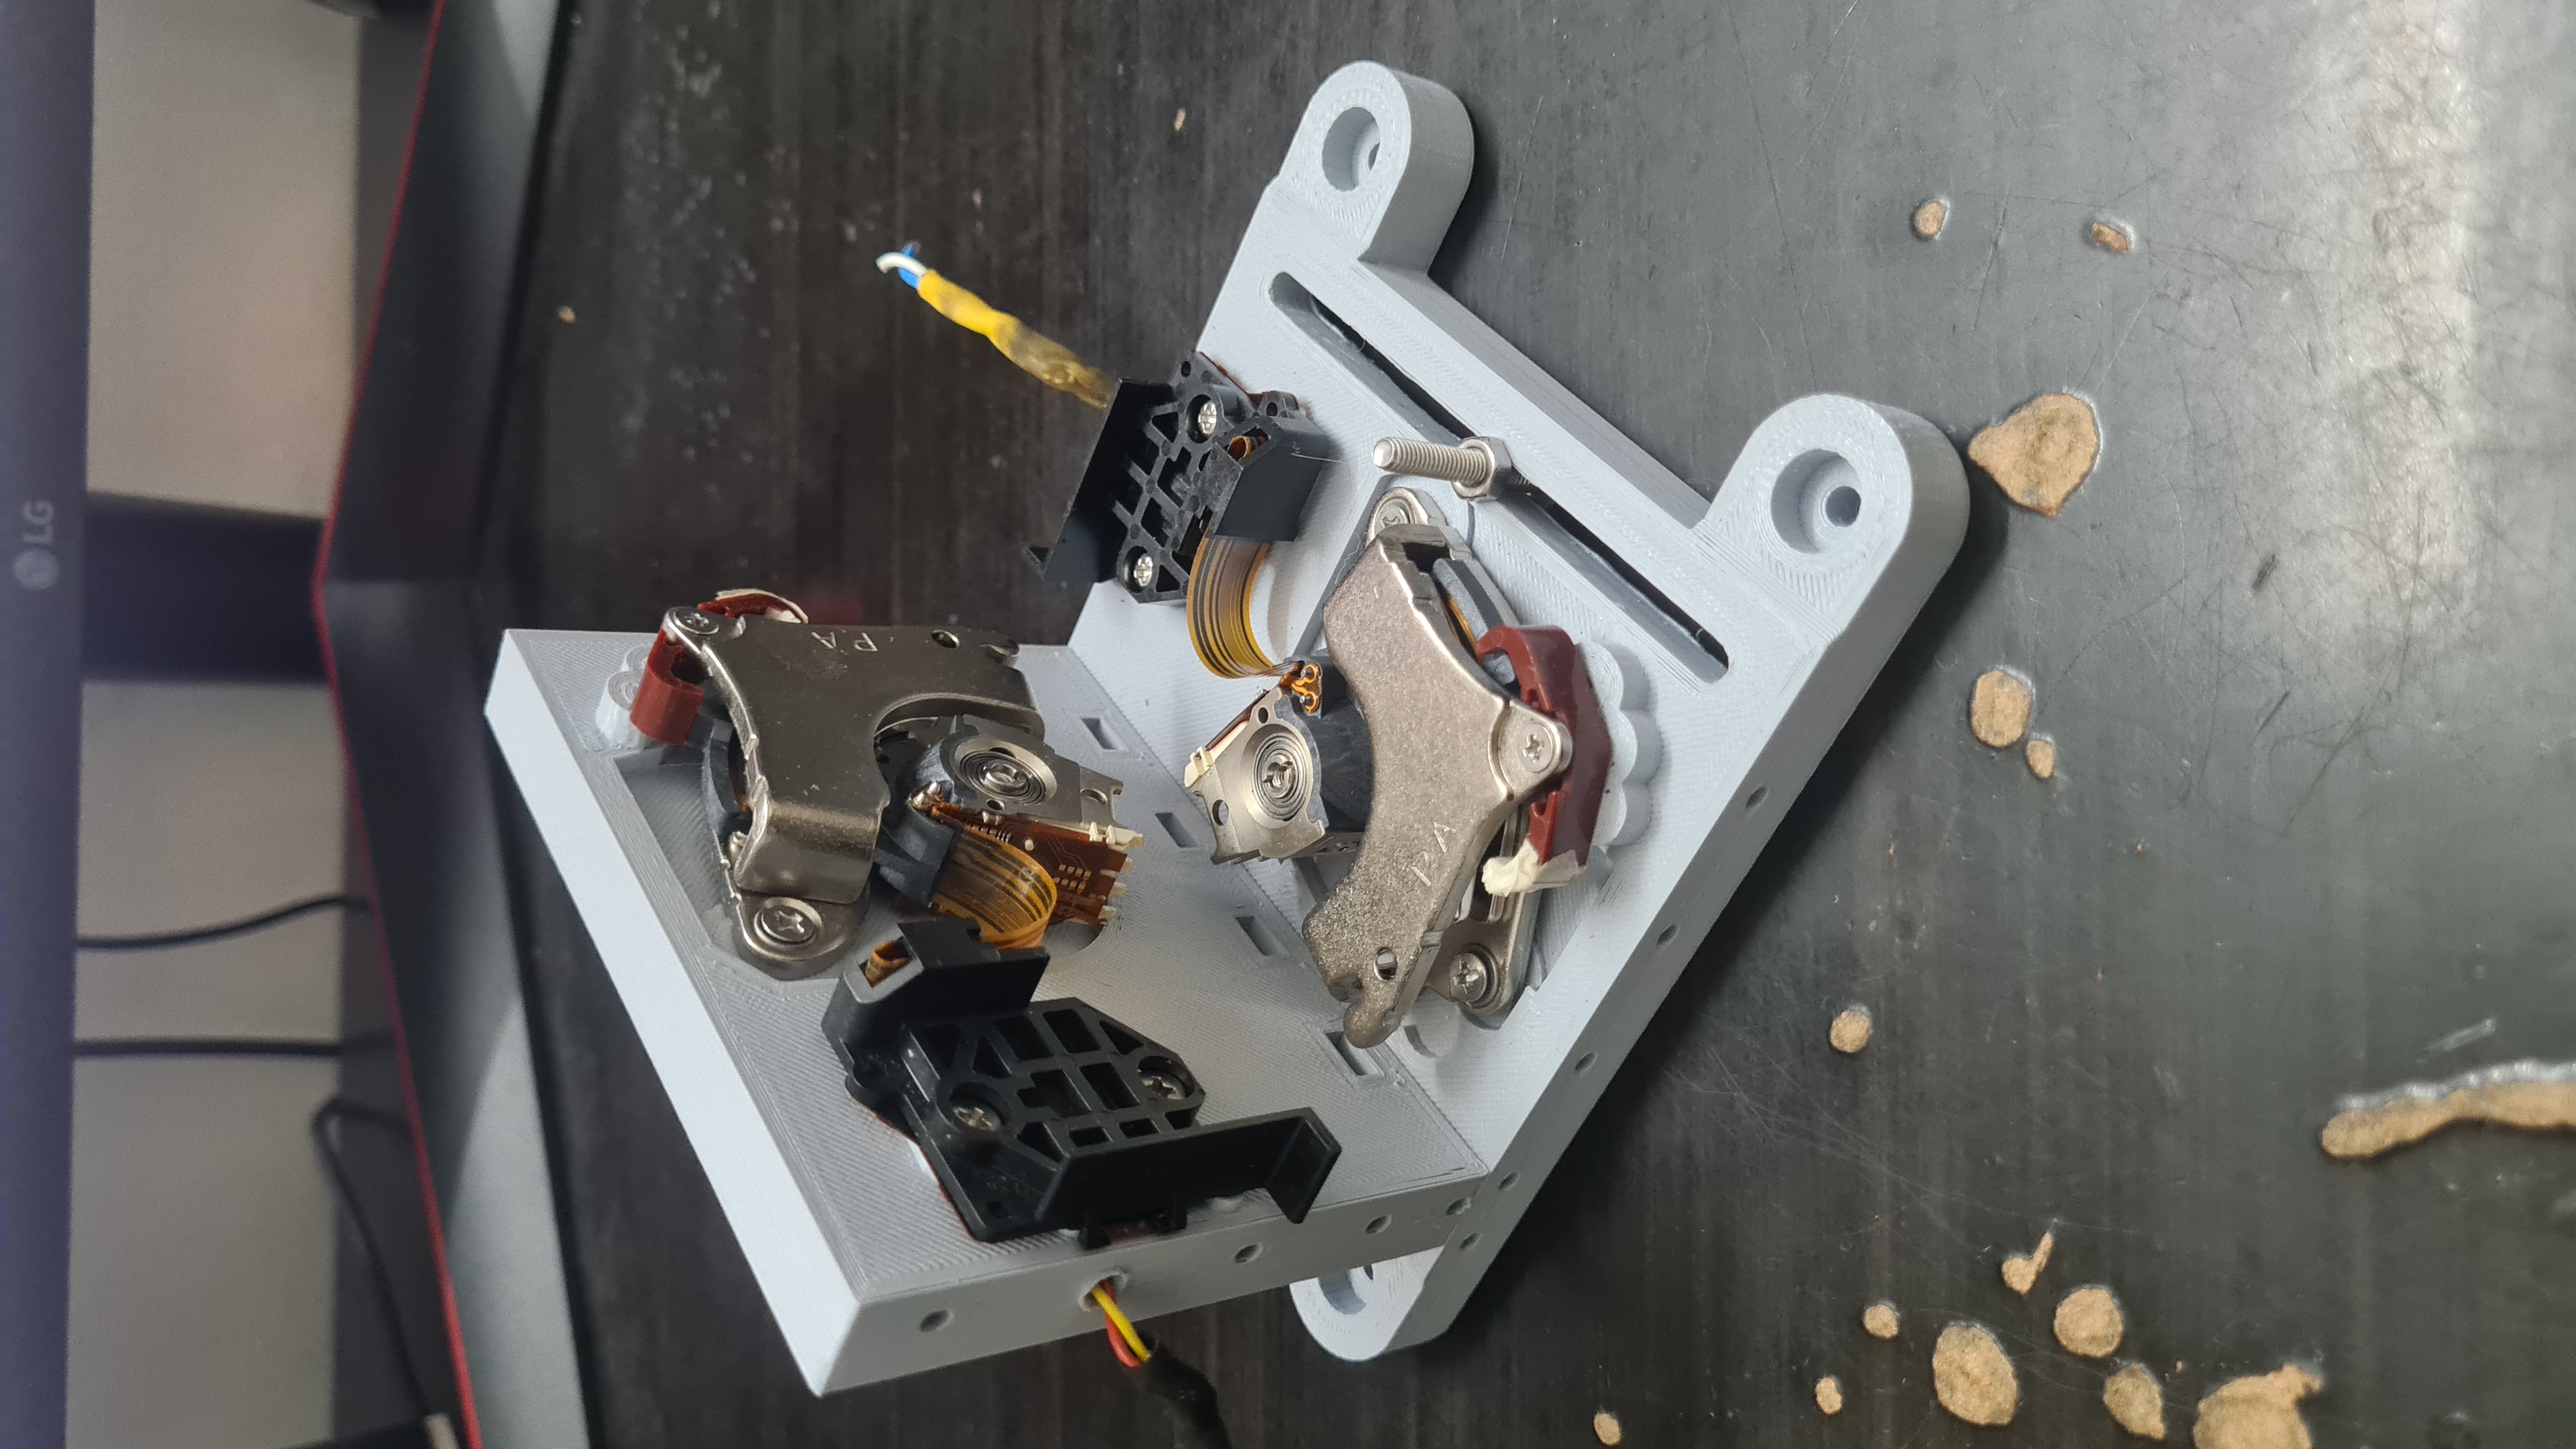
\includegraphics[angle=-90, width=0.85\textwidth,
        trim={25cm 1cm 20cm 1cm}, clip]{./images/11.jpg}
    \caption{Photograph of the 3D-printed dual-axis galvanometer assembly.}
    \label{fig:assembly_prototype}
\end{figure}


\subsection{VCM Mirror Mount: The Decoupled Slotted-Plate Solution}

The core of the mechanical design addresses the kinematic mounting paradox, wherein the mirror's reflective surface must lie on the actuator's pivot axis, a volume physically occupied by the bearing assembly. To resolve this, a \textbf{decoupled, slotted-plate mounting system} was designed.

This system consists of a stationary plate, fabricated from the chosen polymer, which is mounted to the VCM's fixed base. A precision slot, with its centerline designed to be perfectly collinear with the VCM's axis of rotation, provides a rigid, kinematically correct guide for the mirror element. The moving arm of the VCM actuates the mirror via a small, custom-designed fork. This architecture provides superior geometric accuracy and rigidity compared to a cantilevered bracket by separating the function of alignment (handled by the stationary plate) from the function of actuation (handled by the moving arm).

% INSERT FIGURE: VCM Mount Design
\begin{figure}[H]
\centering
% \includegraphics[width=0.8\textwidth]{./images/your_vcm_mount_cad.png} % Replace with your filename
\caption{Detailed view of the custom slotted-plate mirror mount. The stationary plate provides a precise guide for the mirror, ensuring its reflective surface remains on the pivot axis.}
\label{fig:vcm_mount}
\end{figure}

\subsection{Material Selection and Thermal Management Strategy}

The selection of the fabrication material involved a critical trade-off analysis between mechanical performance and thermal stability. The primary heat sources are the VCM coils, which can reach elevated temperatures during high-duty cycle operation.

\subsubsection{Material Choice}
A \textbf{PLA+ (Professional PLA)} filament was selected for all 3D printed structural components. This decision prioritizes the material's superior mechanical properties at ambient temperatures. The higher Young's Modulus (stiffness) and lower susceptibility to creep under static load compared to other FDM materials like PETG are critical for maintaining the long-term dimensional stability and precision of the kinematic mounts and mirror alignment slots.

\subsubsection{Thermal Management}
To mitigate the risk of thermal deformation associated with PLA+'s low glass transition temperature (approx. 60°C), a \textbf{thermal break} is integrated into the mounting design. The VCM assemblies are mounted via metal standoffs, creating an insulating air gap that minimizes heat transfer to the PLA+ baseplate. Furthermore, thin \textbf{polyimide (Kapton) tape washers} are used at the screw-standoff interfaces. Kapton tape is a high-performance polymer film that serves as both a superior electrical insulator and a robust thermal insulator, effectively blocking the conductive heat path through the mounting screws. This strategy allows the system to leverage the mechanical benefits of PLA+ while ensuring thermal stability during operation.


\subsection{Optical Component Sizing and Scope}

To ensure the full angular scan range is achieved without beam clipping (vignetting), the minimum required dimensions for the mirrors were calculated. These calculations are based on the system's geometry and do not extend to lens design, beam focusing, or power density analysis; the optical design is confined to the geometric Line-of-Sight (LOS) stabilization.

\subsubsection{Definitions}
\begin{itemize}
\item \(D_{beam}\): The diameter of the incoming laser beam at the first mirror.
\item \(e\): The inter-mirror pivot distance, obtained from the CAD model.
\item \(\theta_{y,mech}\): The maximum mechanical rotation angle of the X-mirror.
\item \(\alpha_{inc}\): The angle of incidence of the beam on the mirrors (typically 45°).
\item \(S_m\): A safety margin factor (e.g., 1.2 for a 20\% margin).
\end{itemize}

\subsubsection{X-Mirror (First Mirror) Dimensions}
The X-mirror must intercept the stationary incoming beam. The beam's circular cross-section projects as an ellipse onto the tilted mirror surface.
\begin{align}
W_x &= S_m \cdot D_{beam} \\
L_x &= S_m \cdot (D_{beam} / \cos(\alpha_{inc}))
\end{align}
Where \(W_x\) is the minimum width and \(L_x\) is the minimum length.

\subsubsection{Y-Mirror (Second Mirror) Dimensions}
The Y-mirror is more complex as it must intercept a beam that is already being scanned by the X-mirror. Its dimensions must account for the beam's footprint plus the full length of the scanned line.
\begin{align}
W_y &= S_m \cdot \left[ (D_{beam} / \cos(\alpha_{inc})) + (2 \cdot e \cdot \tan(\theta_{y,mech})) \right] \\
L_y &= S_m \cdot (D_{beam} / \cos(\alpha_{inc}))
\end{align}
Where \(W_y\) is the minimum width (along its pivot axis) and \(L_y\) is the minimum length. The length \(L_y\) is determined by the beam footprint, as the primary scan occurs along the width \(W_y\). A more rigorous model would include second-order effects on \(L_y\), but for small angles, they are negligible.

These calculations provide the minimum required clear aperture for the optical elements, guiding the selection and fabrication of the mirrors from HDD platter stock.

\subsection{Optical Component Sizing for Maximum Scan Range}

A critical aspect of the mechanical design is the determination of the minimum required mirror dimensions to prevent beam clipping (vignetting) across the full operational range of the actuators. An insufficient mirror size would act as a mechanical aperture, limiting the achievable scan field. The following analysis calculates the minimum required clear aperture for both the X and Y-axis mirrors based on the system's specified geometry and maximum angular deflection.

\subsubsection{System Parameters and Definitions}
The calculations are based on the following system parameters, derived from component datasheets, the CAD model, and the project's operational requirements:

\begin{itemize}
\item \textbf{Actuator Mechanical Range (\(\theta_{mech,max}\))}: The VCM actuators have a total mechanical range of 30°, corresponding to a maximum deflection from the center position of \(\pm 15^\circ\). Therefore, \(\theta_{mech,max} = 15^\circ\).
\item \textbf{Laser Beam Diameter (\(D_{beam}\))}: The laser module produces a beam with an approximate diameter of 2.0 mm.
\item \textbf{Inter-Mirror Pivot Distance (\(e\))}: The distance between the X-mirror and Y-mirror pivot axes, as determined from the CAD assembly, is 15.0 mm.
\item \textbf{Angle of Incidence (\(\alpha_{inc}\))}: For a standard orthogonal layout, the beam angle of incidence on each mirror surface is 45°.
\item \textbf{Safety Margin (\(S_m\))}: A safety margin of 1.2 (20\%) is applied to all calculations to account for minor misalignments and beam divergence.
\end{itemize}

\subsubsection{X-Mirror (First Mirror) Dimension Calculation}
The first mirror must be large enough to intercept the stationary incoming beam. The beam's circular cross-section of diameter \(D_{beam}\) projects as an ellipse onto the mirror surface, which is tilted at \(\alpha_{inc}\).

The minimum required width (\(W_x\)) and length (\(L_x\)) are given by:
\begin{align}
W_x &= S_m \cdot D_{beam} \\
L_x &= S_m \cdot (D_{beam} / \cos(\alpha_{inc}))
\end{align}

Substituting the system parameters:
\begin{align}
W_x &= 1.2 \cdot 2.0\,\text{mm} = 2.4\,\text{mm} \\
L_x &= 1.2 \cdot (2.0\,\text{mm} / \cos(45^\circ)) \approx 1.2 \cdot (2.0\,\text{mm} / 0.707) \approx 3.4\,\text{mm}
\end{align}
Therefore, the minimum required clear aperture for the X-mirror is \textbf{2.4 mm x 3.4 mm}.

\subsubsection{Y-Mirror (Second Mirror) Dimension Calculation}
The second mirror is more complex as it must intercept a beam that is already being scanned by the first mirror. Its width must account for both the beam's own footprint and the full linear sweep produced by the X-mirror's rotation.

The minimum required width (\(W_y\)) along its pivot axis is given by:
\begin{equation}
W_y = S_m \cdot \left[ (D_{beam} / \cos(\alpha_{inc})) + (2 \cdot e \cdot \tan(\theta_{y,mech,max})) \right]
\end{equation}
The minimum required length (\(L_y\)) is determined by the beam footprint, as the primary scan occurs along the width:
\begin{equation}
L_y = S_m \cdot (D_{beam} / \cos(\alpha_{inc}))
\end{equation}

Substituting the system parameters into the equation for the critical width \(W_y\):
\begin{align}
W_y &= 1.2 \cdot \left[ (2.0\,\text{mm} / \cos(45^\circ)) + (2 \cdot 15.0\,\text{mm} \cdot \tan(15^\circ)) \right] \\
W_y &= 1.2 \cdot [ 2.83\,\text{mm} + (30.0\,\text{mm} \cdot 0.2679) ] \\
W_y &= 1.2 \cdot [ 2.83\,\text{mm} + 8.04\,\text{mm} ] = 1.2 \cdot [10.87\,\text{mm}] \approx 13.04\,\text{mm}
\end{align}
The length calculation remains the same: \(L_y \approx 3.4\,\text{mm}\).

Therefore, the minimum required clear aperture for the Y-mirror is \textbf{13.1 mm x 3.4 mm}. These dimensions will be used for the fabrication of the mirrors from HDD platter stock to ensure the system can achieve its maximum theoretical scan range without vignetting.

\subsubsection{Maximum Scan Field Calculation}
The maximum scan field is determined by the maximum optical deflection angle, which is a direct consequence of the actuator's mechanical range due to the 2\(\theta\) rule.

\begin{equation}
\theta_{opt,max} = 2 \cdot \theta_{mech,max} = 2 \cdot 15^\circ = 30^\circ
\end{equation}

The maximum linear displacement (\(X_{max}\)) from the center of the screen along a single axis is given by the planar projection formula:
\begin{equation}
X_{max} = d \cdot \tan(\theta_{opt,max})
\end{equation}

Substituting the system parameters:
\begin{align}
X_{max} &= 500\,\text{mm} \cdot \tan(30^\circ) \\
X_{max} &\approx 500\,\text{mm} \cdot 0.57735 \approx 288.7\,\text{mm}
\end{align}

The total width of the scan field is twice this maximum displacement. This results in a theoretical maximum scan area at the 50 cm projection distance of approximately \textbf{57.7 cm x 57.7 cm}. This large field of view confirms that the VCM actuators provide a sufficient angular range for a wide variety of applications.

\newpage
% ===================================================================
% CHAPTER 3: SYSTEM DYNAMICS AND CONTROL
% ===================================================================
\section{System Dynamics and Control}

While the kinematic model describes the geometry of the laser steering system, the dynamic model describes its behavior over time in response to inputs. For high-performance control, especially for disturbance rejection, it is advantageous to move beyond simple transfer functions and describe the system's internal dynamics using a state-space representation.

\subsection{State-Space Representation}

State-space modeling provides a complete description of a system's internal state in a first-order matrix form. This representation is powerful for multi-input, multi-output (MIMO) systems and is the foundation for modern control techniques like LQR and state estimators like the Kalman filter.

The standard form is given by two equations:
\begin{align}
    \dot{\mathbf{x}}(t) &= \mathbf{A}\mathbf{x}(t) + \mathbf{B}\mathbf{u}(t) \label{eq:state_equation} \\
    \mathbf{y}(t) &= \mathbf{C}\mathbf{x}(t) + \mathbf{D}\mathbf{u}(t) \label{eq:output_equation}
\end{align}

Where:
\begin{itemize}
    \item \(\mathbf{x}(t)\) is the \textbf{state vector}. This is the minimal set of variables needed to fully describe the system's internal state at time \(t\). For a single mechanical axis (one motor), this vector typically includes angular position (\(\theta\)) and angular velocity (\(\dot{\theta}\)).
    \begin{equation*}
        \mathbf{x} = \begin{bmatrix} \theta \\ \dot{\theta} \end{bmatrix}
    \end{equation*}

    \item \(\mathbf{u}(t)\) is the \textbf{input vector}. This represents the external signal used to control the system. In our case, this is the voltage applied to the motor driver.

    \item \(\mathbf{y}(t)\) is the \textbf{output vector}. This represents the signals that can be physically measured by sensors.

    \item \(\mathbf{A}\) is the \textbf{state matrix}. It describes the system's internal dynamics (how the state evolves on its own, without any input). For a 2x2 matrix, it relates position and velocity.

    \item \(\mathbf{B}\) is the \textbf{input matrix}. It describes how the input signal influences the state (e.g., how input voltage creates an angular acceleration).

    \item \(\mathbf{C}\) is the \textbf{output matrix}. It describes which parts of the state vector are directly measured to form the output vector \(\mathbf{y}\).

    \item \(\mathbf{D}\) is the \textbf{feedthrough matrix}. It represents any direct connection from the input to the output. For most mechanical systems, this is a zero matrix.
\end{itemize}

The matrices \(\mathbf{A}\), \(\mathbf{B}\), and \(\mathbf{C}\) contain the physics of the system. While they can be derived from first principles, a more practical approach for a complex assembly is to determine them experimentally through a process called \textbf{system identification}.

\subsection{Controllability}
Before designing a controller, we must answer a fundamental question: is the system controllable? Controllability asks: "Is it physically possible to drive the system from any initial state to any desired final state in a finite amount of time using the input signal \(\mathbf{u}\)?"

Mathematically, a linear time-invariant (LTI) system is controllable if and only if the \textbf{controllability matrix}, \(\mathcal{C}\), has full rank. For our second-order system, the matrix is:
\begin{equation}
    \mathcal{C} = \begin{bmatrix} \mathbf{B} & \mathbf{AB} \end{bmatrix}
\end{equation}
If \(\det(\mathcal{C}) \neq 0\), the system is controllable, and we can proceed with designing a controller that can fully manipulate its state.

\subsection{Observability}
The dual concept to controllability is observability. It asks: "By observing the output \(\mathbf{y}\) over a period of time, can we uniquely determine the initial state \(\mathbf{x}(0)\)?" In essence, can we deduce the full internal state of the system by looking at its sensor outputs?

Observability is a prerequisite for state estimation. A system is observable if and only if the \textbf{observability matrix}, \(\mathcal{O}\), has full rank. The observability matrix is constructed as:
\begin{equation}
    \mathcal{O} = \begin{bmatrix} \mathbf{C} \\ \mathbf{CA} \end{bmatrix}
\end{equation}
If \(\det(\mathcal{O}) \neq 0\), the system is observable. This means we can design a state estimator, like a Kalman filter, to reconstruct the full state vector (e.g., estimate velocity from position measurements).

\subsection{The Control Workflow: A Full Picture}
The state-space model, along with the concepts of controllability and observability, forms a powerful and cohesive workflow for system control:
\begin{enumerate}
    \item Perform \textbf{System Identification} on the physical hardware to obtain the matrices \(\mathbf{A}\), \(\mathbf{B}\), and \(\mathbf{C}\) that mathematically describe the galvanometer dynamics.
    \item Check the \textbf{controllability} and \textbf{observability} matrices to prove that the system is well-designed and that a state-feedback controller and estimator are feasible.
    \item Implement a \textbf{Kalman Filter} using the system model (\(\mathbf{A, B, C}\)) to produce an optimal estimate of the full state \(\mathbf{x}\) (position and velocity) from noisy sensor data.
    \item Feed this clean state estimate into a state-feedback controller (like an \textbf{LQR controller}) that uses the state matrices to calculate the optimal motor voltage required to drive the system to its target state.
    \item This entire low-level control loop receives its high-level goals (the desired mirror angles \(\theta_x, \theta_y\)) from the numerical \textbf{Inverse Kinematics solver}.
\end{enumerate}

\newpage

% ===================================================================
% CHAPTER 4: OBJECTIVES AND METHODOLOGY
% ===================================================================
\section{Project Objectives}

The primary goal of this research is to design, build, and validate a low-cost, high-performance laser steering system capable of precise targeting and active vibration compensation on mobile platforms. The specific objectives are as follows:

\begin{enumerate}
    \item \textbf{Design and Fabricate a Low-Cost Actuation System:} Develop and construct a functional, dual-axis laser steering system using salvaged mechatronic components (e.g., voice coil motors from HDDs) as a resource-constrained alternative to expensive commercial galvanometers.

    \item \textbf{Develop a Hybrid Sensor Fusion Framework:} Integrate data from an Inertial Measurement Unit (IMU) with vision-based data (optical flow and object tracking) to create a robust, real-time estimate of both platform motion and target location, enabling line-of-sight stabilization.

    \item \textbf{Implement and Compare Advanced Control Strategies:} Derive an accurate state-space model of the system's dynamics via experimental system identification. Based on this model, implement and comparatively analyze the performance of multiple control architectures (PID, LQR, MPC) for stabilization and disturbance rejection.

    \item \textbf{Develop an AI-Powered Visual Servoing Pipeline:} Implement a complete computer vision pipeline for real-time weed detection (YOLOv8), classification, and object tracking (DeepSORT/ByteTrack) to provide dynamic target coordinates to the control system.

    \item \textbf{Experimentally Validate System Performance:} Quantify the system's targeting and stabilization performance under simulated real-world conditions. This involves deploying the system on a motion platform to measure key metrics such as jitter suppression, tracking error, and response time under various dynamic loads.
\end{enumerate}

\section{Proposed Methodology}

The project will be executed in four distinct stages, progressing from hardware fabrication to system-level validation.

\subsection{Stage 1: System Design and Fabrication}
This stage focuses on creating the core physical hardware.
\begin{itemize}
    \item \textbf{Mechanical Design:} A dual-axis galvanometer assembly will be designed using CAD software. The design will focus on optimizing actuation geometry and structural layout to minimize backlash, inertia, and mechanical resonance.
    \item \textbf{Actuator and Optics Sourcing:} Voice coil motors (VCMs) and front-surface mirrors will be salvaged from defunct Hard-Disk Drives (HDDs) or optical disc drives.
    \item \textbf{Electronics Integration:} The mechanical assembly will be integrated with a high-speed microcontroller (e.g., Teensy 4.1), custom motor drivers, an Inertial Measurement Unit (IMU), and an optical flow sensor to form the mechatronic base.
\end{itemize}

\subsection{Stage 2: Modeling and Control System Implementation}
This stage focuses on developing the low-level control intelligence.
\begin{itemize}
    \item \textbf{System Identification:} The dynamic response of the fabricated plant will be characterized. Experimental tests such as step response analysis and frequency sweeps (generating Bode plots) will be performed to gather empirical data.
    \item \textbf{State-Space Modeling:} The empirical data will be used to derive a mathematical state-space model (\(\mathbf{A, B, C}\) matrices) that accurately represents the system's input-output dynamics.
    \item \textbf{Controller Design:} Multiple controllers will be designed and implemented for line-of-sight stabilization based on the identified model, including a classical PID controller and modern state-feedback controllers such as a Linear-Quadratic Regulator (LQR).
\end{itemize}

\subsection{Stage 3: Vision and Sensor Fusion Development}
This stage builds the high-level perception and targeting system.
\begin{itemize}
    \item \textbf{AI-Based Object Detection:} A YOLOv8 model will be trained or fine-tuned on public datasets for robust weed detection.
    \item \textbf{Real-Time Object Tracking:} A tracking algorithm (e.g., DeepSORT or ByteTrack) will be implemented to maintain a persistent identity for each detected target across video frames.
    \item \textbf{Visual-Inertial Fusion:} Algorithms will be developed to fuse the high-frequency motion data from the IMU with the vision-based data (target location, optical flow) to produce a highly accurate, real-time estimate of beam deviation and absolute target location, even during platform motion.
\end{itemize}

\subsection{Stage 4: Experimental Validation and Analysis}
The final stage focuses on testing the integrated system.
\begin{itemize}
    \item \textbf{Testbed Setup:} The complete system will be mounted on a programmable motion platform capable of simulating real-world vibrations and field disturbances.
    \item \textbf{Performance Measurement:} Systematic experiments will be conducted to quantify key performance metrics, including pointing accuracy, tracking error, jitter suppression, and settling time.
    \item \textbf{Comparative Analysis:} The performance and robustness of the different control strategies (PID vs. LQR) will be evaluated and compared under various simulated visual and mechanical workloads.
\end{itemize}

\newpage

\end{document}